\begin{section}{Resultados}

\subsection{Sa�da das Consultas}
\subsubsection{\textbf{Consulta 1}}
	Consulta da Folha de frequ�ncia de todos os estudantes (Figuras ~\ref{fig:r11}
e ~\ref{fig:r12}).
\begin{figure}[!h]
    \centering
    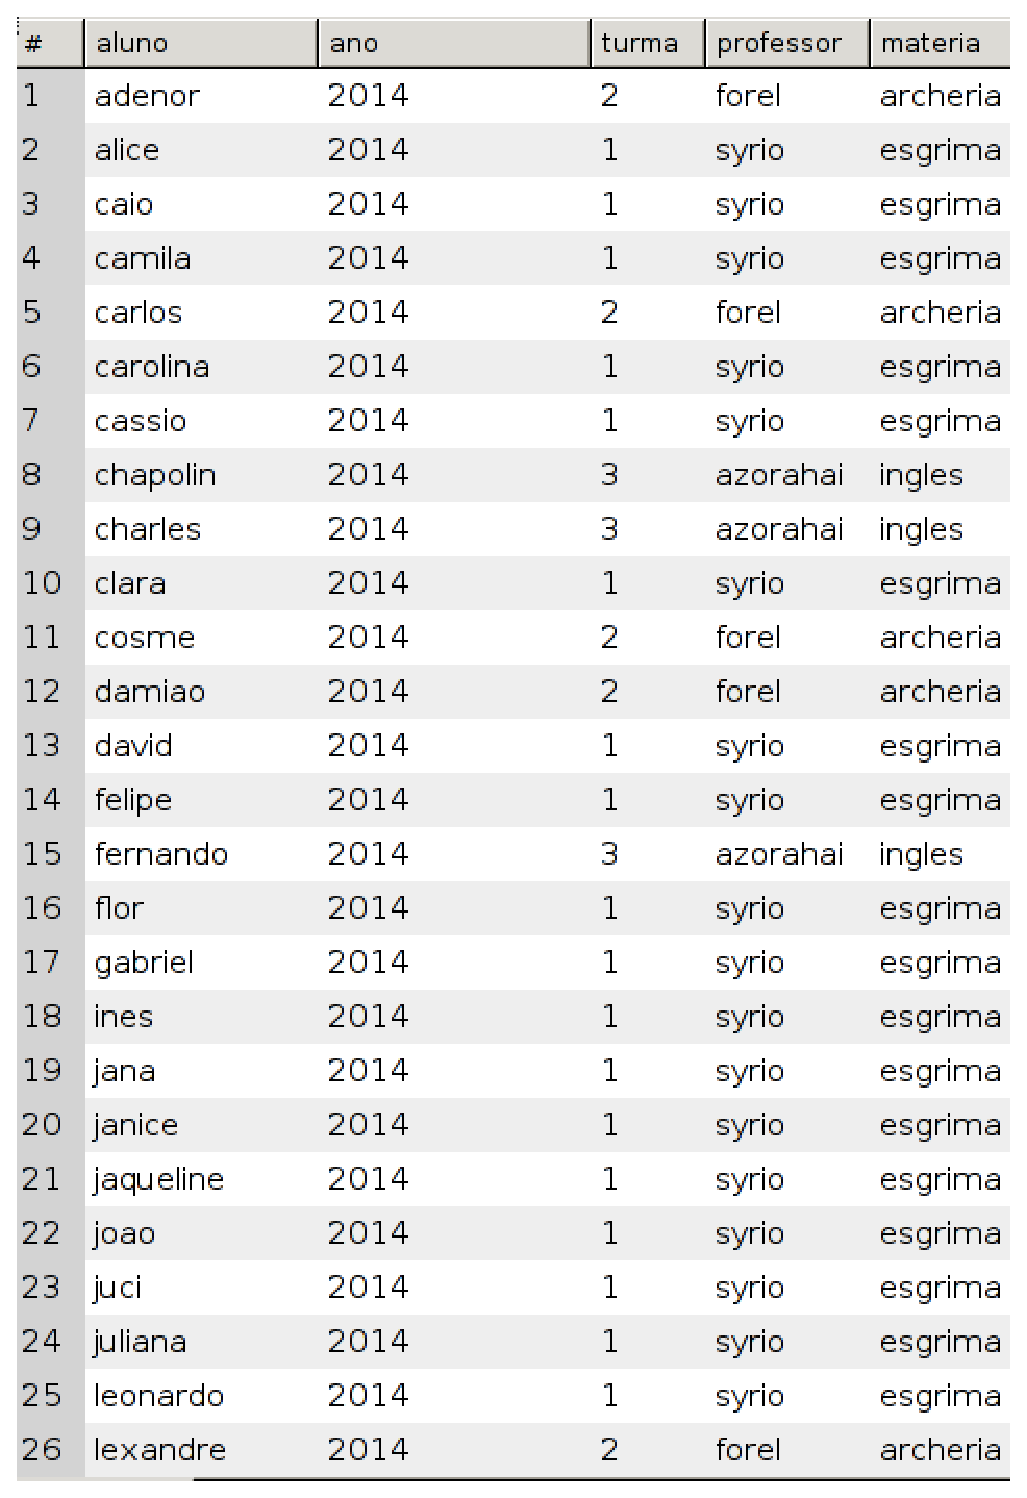
\includegraphics[width=.7\textwidth]{Figures/r11}
    \caption{Sa�da da Consulta 1 \textbf{parte 1}}
    \label{fig:r11}
\end{figure}

\begin{figure}[!h]
    \centering
    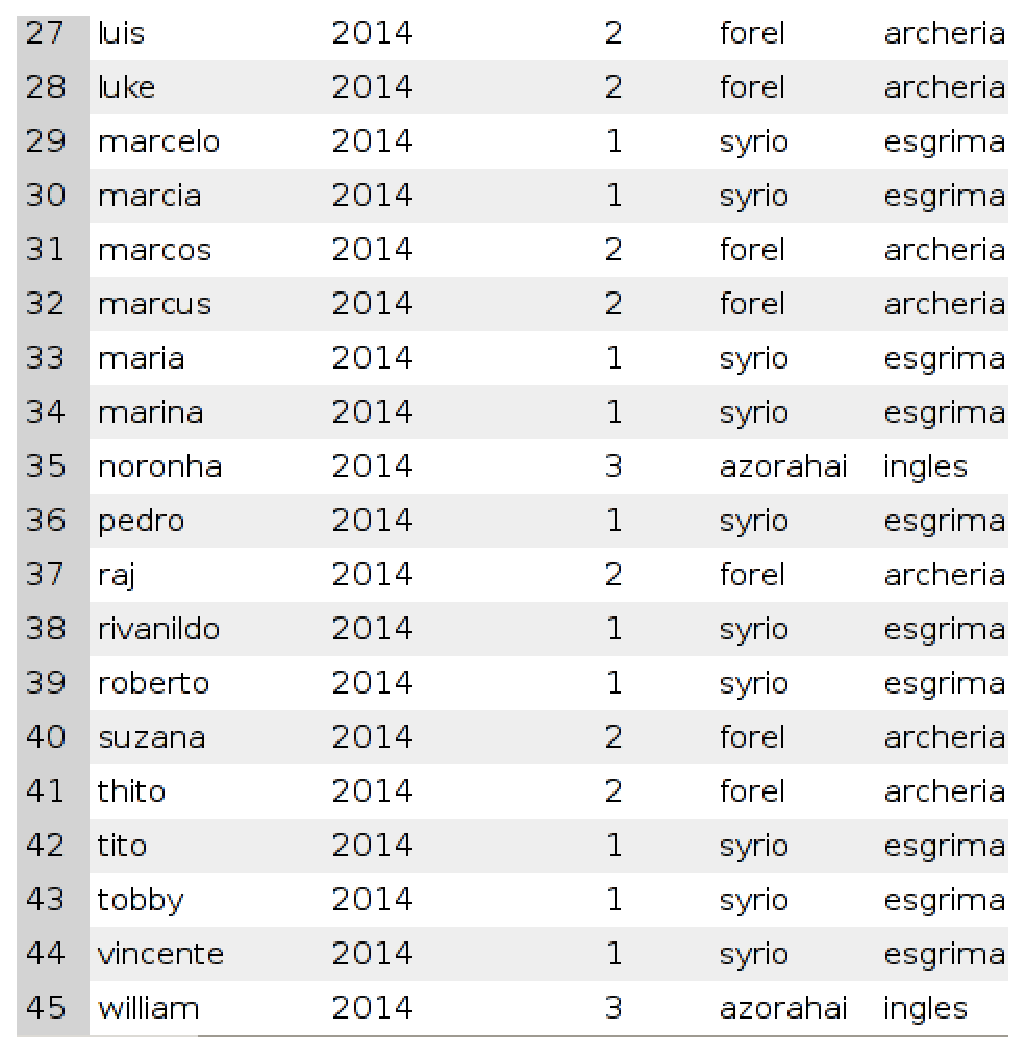
\includegraphics[width=.7\textwidth]{Figures/r12}
    \caption{Sa�da da Consulta 1 \textbf{parte 2}}
    \label{fig:r12}
\end{figure}

\subsubsection{\textbf{Consulta 2}}

	Boletim de notas de alguns estudantes (Figura ~\ref{fig:r2}).
\begin{figure}[!h]
    \centering
    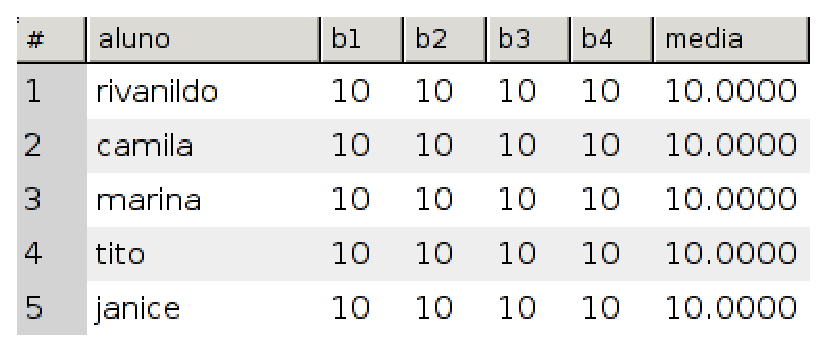
\includegraphics[width=.7\textwidth]{Figures/r2}
    \caption{Sa�da da Consulta 2}
    \label{fig:r2}
\end{figure}

\subsubsection{\textbf{Consulta 3}}
	Hist�rico cumulativo de alguns dos estudantes (Figura ~\ref{fig:r3}).
\begin{figure}[!h]
    \centering
    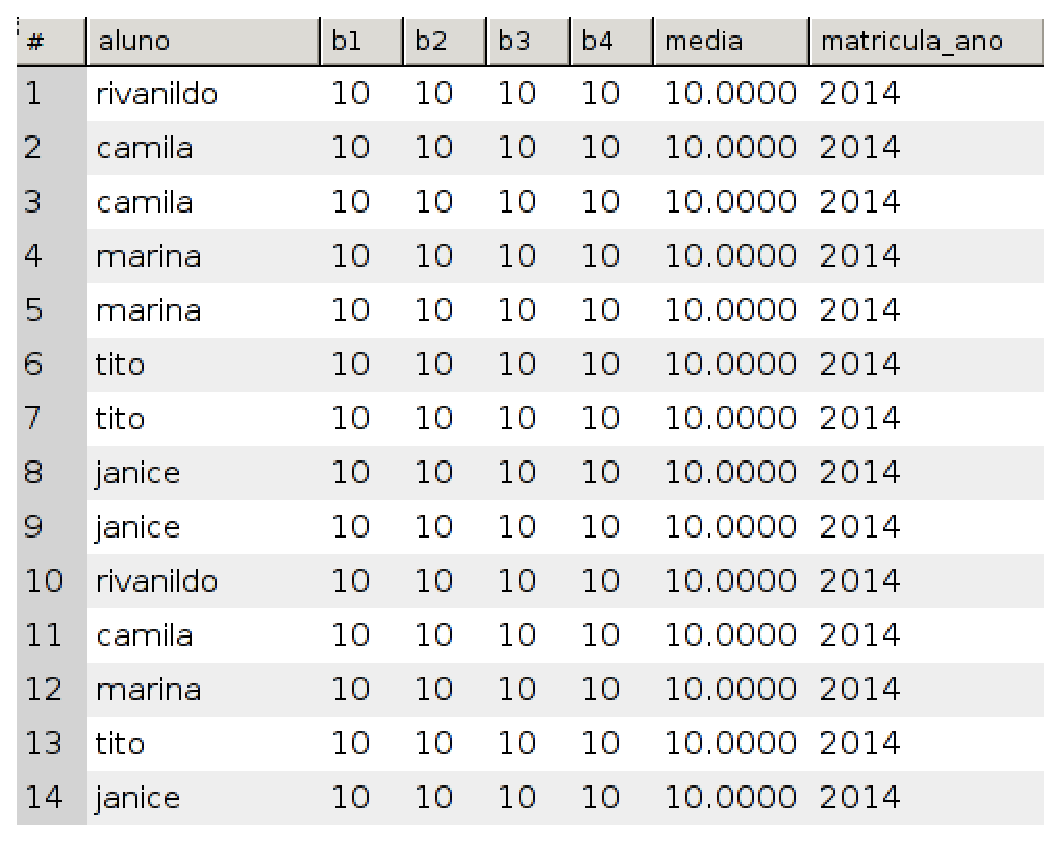
\includegraphics[width=.7\textwidth]{Figures/r3}
    \caption{Sa�da da Consulta 3}
    \label{fig:r3}
\end{figure}

\subsubsection{\textbf{Consulta 4}}
	Nome dos alunos em recupera��o por turma (Figura ~\ref{fig:r4}).
\begin{figure}[!h]
    \centering
    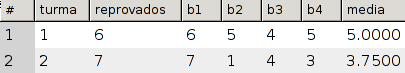
\includegraphics[width=.7\textwidth]{Figures/r4}
    \caption{Sa�da da Consulta 4}
    \label{fig:r4}
\end{figure}

\subsubsection{\textbf{Consulta 5}}
	Boleto mensal de (2) respons�veis (Figura ~\ref{fig:r5}).
\begin{figure}[!h]
    \centering
    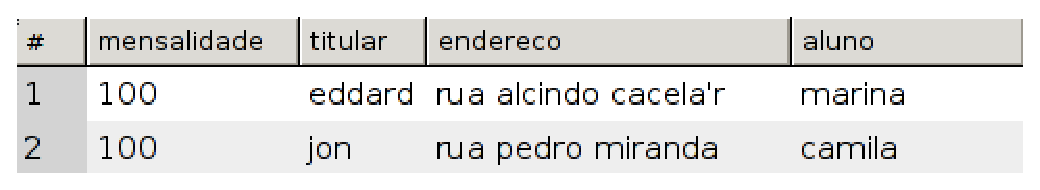
\includegraphics[width=.7\textwidth]{Figures/r5}
    \caption{Sa�da da Consulta 5}
    \label{fig:r5}
\end{figure}

\subsubsection{\textbf{Consulta 6}}
	Extrato anual de (3) alunos (Figura ~\ref{fig:r6}).
\begin{figure}[!h]
    \centering
    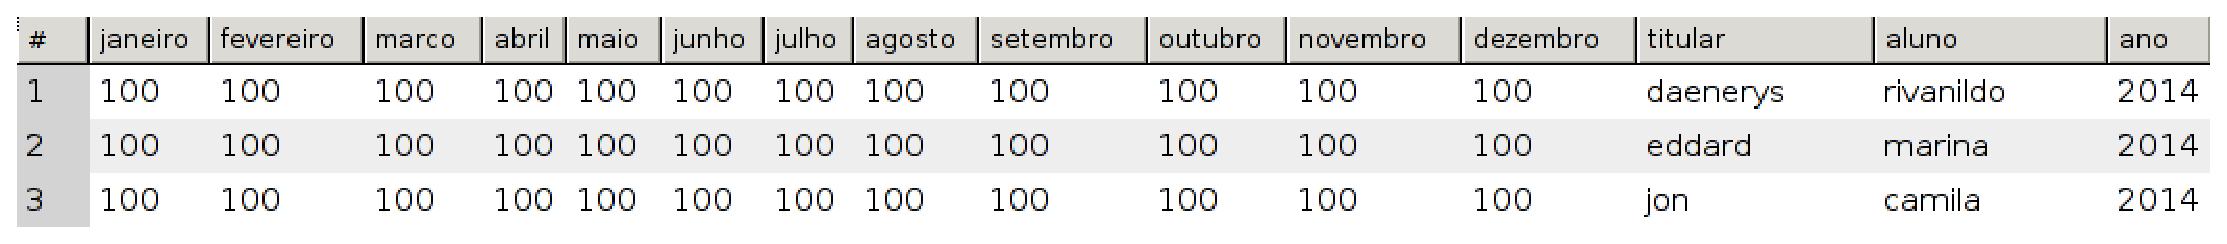
\includegraphics[width=.8\textwidth]{Figures/r6}
    \caption{Sa�da da Consulta 6 }
    \label{fig:r6}
\end{figure}


\end{section}
%%% EOF %%%
